% vim: spell spelllang=en:
\documentclass[12pt, oneside]{article}
\usepackage[a4paper, left=2.5cm, right=2.5cm, top=2.5cm, bottom=2.5cm]{geometry}

\usepackage[utf8]{inputenc} % Use unicode
\usepackage[T1]{fontenc}
\usepackage[english]{babel} % Names in spanish

%% Bibliography:
%\usepackage{comment}
%\usepackage[
    %backend=biber,
    %style=numeric,
%]{biblatex}
%\DeclareNameAlias{default}{last-first}

%\usepackage{csquotes}       % For bibliography quotations
%\DeclareQuoteAlias{spanish}{catalan}

%\addbibresource{biblio.bib}
%% see:
%% https://www.sharelatex.com/learn/Bibliography_management_in_LaTeX#The_bibliography_file

%\usepackage{datetime} % Customize date
%% \monthyeardate\today gives the date without the day
%\newdateformat{monthyeardate}{%
    %\monthname[\THEMONTH], \THEYEAR}

% For cross references
\usepackage[colorlinks = true]{hyperref}
\usepackage[catalan]{varioref}
%\usepackage{cleveref}
%hyperref configuration so that it doesn't contrast so much colorlinks,
\hypersetup{
   linkcolor={black},
   citecolor={black},
   %linkcolor={red!50!black},
   %citecolor={blue!50!black},
   urlcolor={blue!80!black}
}

\usepackage{xcolor}     % color

\usepackage{mathtools}  % amsmath + more
\usepackage{amsthm}     % Theorem enviroment
\usepackage{amssymb}    % More symbols
\usepackage{amstext}    % Text inside mathenv

\usepackage{relsize}    % Bigger math with mathlarger{___}
\usepackage{nicefrac}   % nice fractions in one line

\usepackage[export]{adjustbox}  % Adjust table size
\usepackage{float}              % Force tables and images position (H and H!)
\usepackage{wrapfig}            % Wrap images like in HTML

\usepackage{tabularx, colortbl, booktabs}    % Better tables
\usepackage{longtable}                      % Multiple page table

% Split cell in lines and more formating options inside table
\usepackage{array, multirow, multicol, makecell}

%\usepackage{subcaption}                     % Subfigures
%\usepackage[framemethod=tikz]{mdframed}     % Custom frames

%\usepackage[bottom]{footmisc} % Footnotes at bottom of page

%\usepackage[alsoload=hep]{siunitx}          % SI units and uncertainties
%\sisetup{locale = FR}                       % Commas and so on for spanish
%\sisetup{separate-uncertainty=true}
%\sisetup{
  %per-mode=fraction,
  %fraction-function=\nicefrac
%}

%\usepackage{tikz}
%%\usetikzlibrary{arrows}
%%\usetikzlibrary{scopes}
%\usetikzlibrary{babel}

%\usepackage{listings}       % For code blocks

%% Custom code highlight
%\definecolor{codegreen}{rgb}{0,0.6,0}
%\definecolor{codegray}{rgb}{0.5,0.5,0.5}
%\definecolor{codepurple}{rgb}{0.58,0,0.82}
%\definecolor{backcolour}{rgb}{0.95,0.95,0.92}
%\definecolor{lightblue}{RGB}{135,206,250}

%\lstdefinestyle{mystyle}{ backgroundcolor=\color{backcolour},
    %commentstyle=\color{codegreen}, keywordstyle=\color{blue},
    %numberstyle=\tiny\color{codegray}, stringstyle=\color{red},
    %identifierstyle=\color{black}, basicstyle=\footnotesize,
    %%breakatwhitespace=false,
    %breaklines=true,
    %%captionpos=b,                    keepspaces=true,
    %numbers=left,                    numbersep=5pt,
    %showspaces=false,
    %%showstringspaces=false, showtabs=false,
    %tabsize=4
%}
%\lstset{style=mystyle}

\newcommand{\whitepage}{
    \clearpage\thispagestyle{empty}\addtocounter{page}{-1} \newpage \clearpage
}

% Add command before appendix session for page numbering: A-1
%\newcommand{\appendixpagenumbering}{
    %\break
    %\pagenumbering{arabic}
    %\renewcommand{\thepage}{\thesection-\arabic{page}}
%}

%% Custom Math operators (functions not in italic in math mode):
%\DeclareMathOperator{\arcsec}{arcsec}
%\DeclareMathOperator{\arccot}{arccot}
%\DeclareMathOperator{\arccsc}{arccsc}
%\DeclareMathOperator{\cis}{cis}


\usepackage{caption}
\usepackage{subcaption}
\usepackage{graphicx}
\usepackage{enumitem}
\usepackage{lipsum}

\usepackage{siunitx}
\usepackage{hyphenat}

\usepackage{xcolor}

\definecolor{LightGray}{rgb}{0.83, 0.83, 0.83}
\definecolor{bg}{HTML}{282828}

\usepackage{minted}
\setminted{
style=monokai,
%frame=lines,
framesep=2mm,
baselinestretch=1.2,
breaklines,
bgcolor=bg,
fontsize=\footnotesize,
linenos
}

\renewcommand\theadfont{\bfseries}

\title{
    PAR Laboratory Assignment\\
    Lab 3: Embarrassingly parallelism with OpenMP:\\ Mandelbrot set
}

\author{
    par2109:
    Aleix Boné,
    Alex Herrero
}

\date{
    Spring 2019-20
}

\begin{document}

\thispagestyle{empty}
\clearpage
\setcounter{page}{-1}

\begin{titlepage}
{
    \centering
    \null
    \vfill
    {\Huge \bfseries PAR Laboratory Assignment\par}
    \vspace{3em}
    {\Large {\scshape Lab 3:} Embarrassingly parallelism with OpenMP: \\ Mandelbrot set \par}
    \vfill
\begin{center}
\end{center}
    \vspace{3cm}

    \vfill
    {\raggedleft \Large
        Aleix Boné\\
        Alex Herrero\\
        {\bfseries\ttfamily par2109}\\
        \vspace{4em}
        2020-04-16
        \par}
}
\end{titlepage}


\section{Introduction}%
\label{sec:Introduction}

% copy paste form here to ... 
% (solo he cambbiado el tiempo verbal, no se si hace falta cambiarlo más ya que enrealidad lo que queremos decir al principio es lo mismo que dice el enunciado...) (y bueno he borrado un par de parrafos)
In this laboratory assignment we explored the tasking model in OpenMP to express iterative task decompositions. 
We started by exploring the most appropriate ones by using \emph{Tareador}. The program that we used is the computation of the \emph{Mandelbrot set}, a particular set of points, in the complex domain, whose boundary generates a distinctive and easily recognisable two-dimensional fractal shape.

For each point $c$ in a delimited two-dimensional space, the complex quadratic polynomial recurrence $z_{n+1} = z^2_n + c$ is iteratively applied in order to determine if it belongs or not to the Mandelbrot set.  The point is part of the Mandelbrot set if, when starting with $z_0 = 0$ and applying the iteration repeatedly, the absolute value of $z_n$ never exceeds a certain number however large $n$ gets.

We analyzed the potential parallelism for two possible task granularities that can be exploited in this program. Those two are:
\begin{enumerate}[label=\alph*)]
\item \emph{Point}: a task corresponds with the computation of a single point (\texttt{row},\texttt{col}) of the Mandelbrot set.
\item \emph{Row}: a task corresponds with the computation of a whole \texttt{row} of the Mandelbrot set.
\end{enumerate}
% ... here

We executed both, \texttt{mandel-tar}\footnote{\texttt{mandel}: used for timing purposes and to check for the numerical validity of the output (non-graphical version).} and \texttt{mandeld-tar}\footnote{\texttt{mandeld}: generates a binary that visualizes the Mandelbrot set (graphical version).}, programs with the different granularities using the \texttt{./run-tareador.sh} script and we obtained the following results.

\begin{figure}[H]
\centering

\includegraphics[width=\textwidth]{plots/dependency_graph_mandel_point.png}
\caption{Task dependence graph of \texttt{mandel-tar.c} with point decomposition.}
\label{graph:mandel_point}
\end{figure}

\begin{figure}[H]
\centering
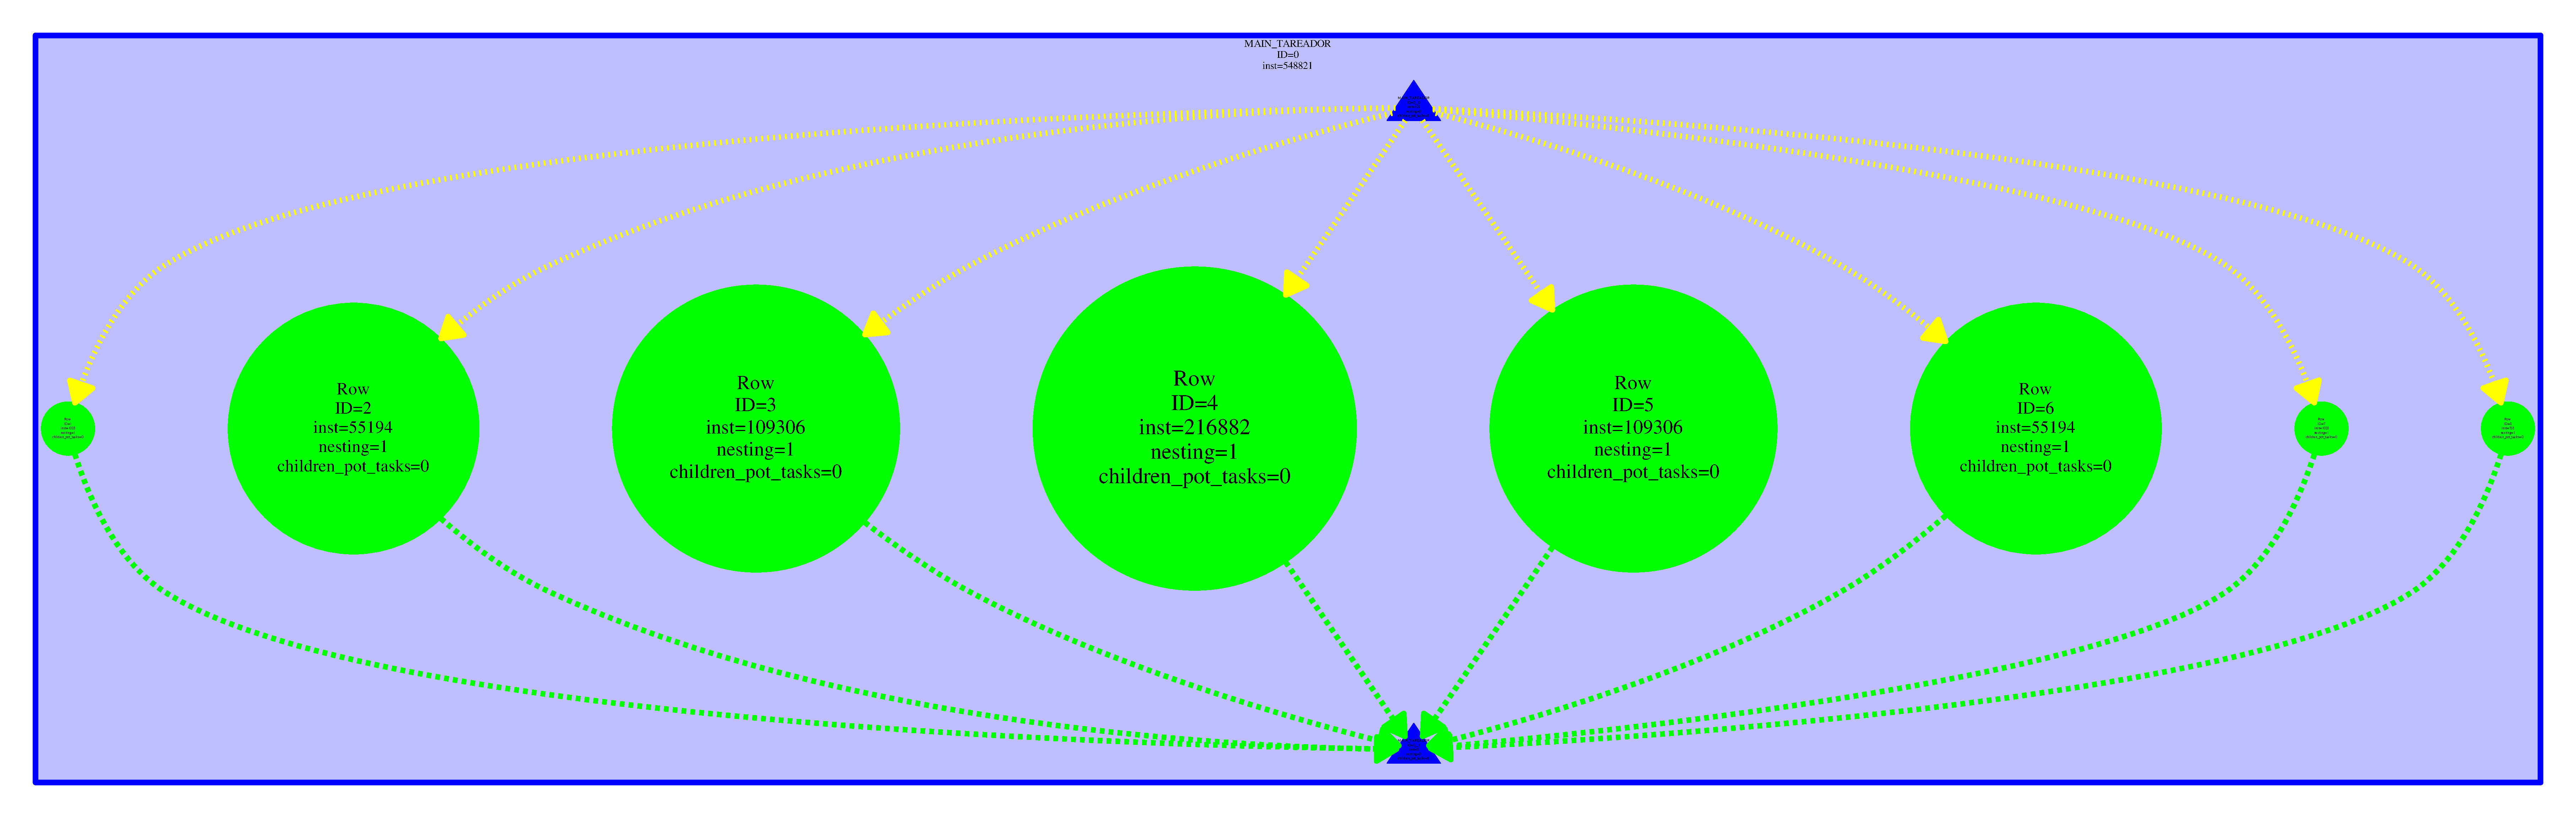
\includegraphics[width=0.6\textwidth]{plots/dependency_graph_mandel_row.pdf}
\caption{Task dependence graph of \texttt{mandel-tar.c} with row decomposition.}
\label{graph:mandel_row}
\end{figure}

% Which are the two most important common characteristics of the task graphs generated for the two task granularities (Point and Row) for the non-graphical version of mandel-tar?  Why the task graphs generated for mandel-tar and mandeld-tar are so different?  Which section of the code do you think is causing the serialization of all tasks in the graphical version?  How will you protect this section of code in the parallel OpenMP code in the next sections?

As we expected the point decomposition has a much more big granularity than the row one. But we obtained that the two decompositions generate similar task graphs for each executable.

We can observe in figures~\ref{graph:mandel_point} and~\ref{graph:mandel_row} that with the \texttt{mandel} executable all tasks can parallelize at the same level. But in figure~\ref{graph:mandeld_point_and_row} we see that with the \texttt{mandeld} executable we obtain a serialization of all tasks.

\begin{figure}[H]
\centering

\includegraphics[height=8cm]{plots/dependency_graph_mandeld_point.png}
\hspace{5em}
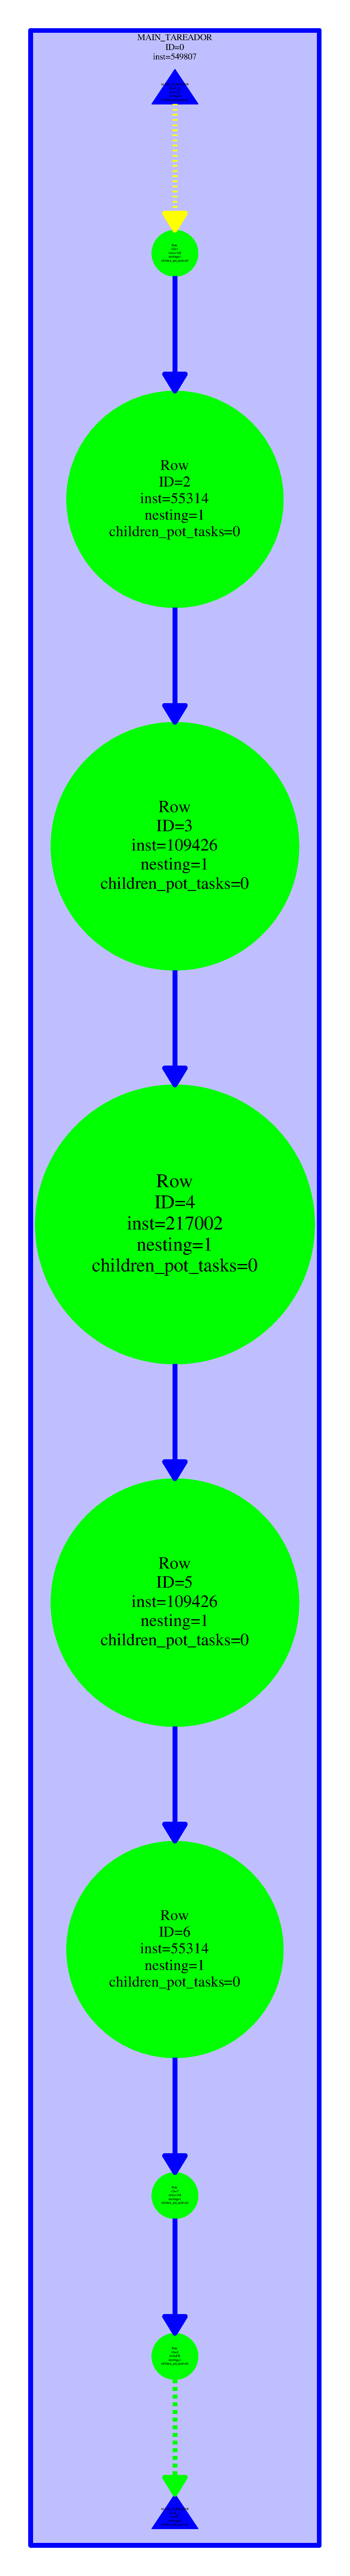
\includegraphics[height=8cm]{plots/dependency_graph_mandeld_row.pdf}
\caption{Task dependence graph of \texttt{mandeld-tar.c} with point and row decompositions.}
\label{graph:mandeld_point_and_row}
\end{figure}

This serialization in the graphical version is caused in the lines 120-130 of the code due to a data race problem that implies full dependence between all tasks. This section can be protected with the \texttt{\#pragma omp critical} clause as shown in the listing~\ref{listing:mandel-omp-critical}.

\begin{listing}[H]
\inputminted[firstline=120,lastline=130]{c}{sources/mandel-omp-v1.c}
\caption{Problematic section in \texttt{mandel-tar.c} protected with \texttt{\#pragma omp critical}.}
\label{listing:mandel-omp-critical}
\end{listing}

% Reason which one of the two task granularities would be more appropriate to apply to implement a parallel version of the Mandelbrot code.
The program is embarrassingly parallelizable so to implement a parallel version of the Mandelbrot code the point granularity should be more appropriate. But with a low number of threads the overhead of task creation would increase and in that case the row granularity could have a better final execution time.

\section{Parallelization Strategies}%
\label{sec:Parallelization Strategies}

%TODO: aqui explicas las strategias del 4.2, 4.3 y 4.4

%$ OMP_NUM_THREADS=1 ./mandeld-omp -i 10000
%Total execution time: 3.228077s
%$ ./mandeld -i 10000
%Total execution time: 3.061886s
%$ OMP_NUM_THREADS=8 ./mandeld-omp -i 10000
%Total execution time: 1.210712s

\section{Performance evaluation}%
\label{sec:Performance evaluation}

%TODO: Aqui comparas



\subsection{\emph{Point} startegy using \emph{OpenMP} \texttt{task}}%

There are multiple ways to create a task for the computation of each point in the Mandelbrot set. We tried
several options and analyzed the performance of each one.

The first version is shown in listing~\ref{lst:v1}. We create a task for each iteration of the \texttt{col} for. The
pool of threads is initialized at every row.

\begin{figure}[H]
    \centering
    \caption{v1 of point task decomposition}
    \inputminted[firstline=91,lastline=98]{c}{sources/mandel-omp-v1.c}
    \label{lst:v1} 
\end{figure}

\begin{figure}[H]
    \centering
    \caption{v2: point task decomposition with taskwait}
    \inputminted[firstline=91,lastline=98]{c}{sources/mandel-omp-v2.c}
    \vspace{-2em}
    \inputminted[firstline=132,lastline=134]{c}{sources/mandel-omp-v2.c}
    \label{lst:v2} 
\end{figure}

\begin{figure}[H]
    \centering
    \caption{v3: point task decomposition with taskgroup}
    \inputminted[firstline=91,lastline=98]{c}{sources/mandel-omp-v3.c}
    \vspace{-2em}
    \inputminted[firstline=133,lastline=135]{c}{sources/mandel-omp-v3.c}
    \label{lst:v3} 
\end{figure}

\begin{figure}[H]
    \centering
    \caption{v4: point task decomposition task without wait}
    \inputminted[firstline=91,lastline=98]{c}{sources/mandel-omp-v4.c}
    \vspace{-2em}
    \inputminted[firstline=131,lastline=133]{c}{sources/mandel-omp-v4.c}
    \label{lst:v4} 
\end{figure}

\begin{figure}[H]
    \centering
    \caption{v5: point task decomposition with taskloop}
    \inputminted[firstline=91,lastline=98]{c}{sources/mandel-omp-v5.c}
    \label{lst:v5} 
\end{figure}

\begin{figure}[H]
    \centering
    \caption{v6: point task decomposition with taskloop grainsize(1)}
    \inputminted[firstline=91,lastline=98]{c}{sources/mandel-omp-v6.c}
    \label{lst:v6} 
\end{figure}

\begin{figure}[H]
    \centering
    \caption{v7: point task decomposition with taskloop grainsize(1) nogroup}
    \inputminted[firstline=91,lastline=98]{c}{sources/mandel-omp-v7.c}
    \label{lst:v7} 
\end{figure}

\begin{figure}[H]
    \centering
    \caption{v8: row task decomposition}
    \inputminted[firstline=91,lastline=98]{c}{sources/mandel-omp-v8.c}
    \label{lst:v7} 
\end{figure}

%
%lo estoy metiendo aqui de momento.
%
%%%%%%%%%%%%%%%%%%%%%%%%%%%%%%%%%%%%%%%%%%%%%%%%%%%%%%%%%%%%

\begin{figure}[H]
    \begin{minipage}{0.5\textwidth}
        \centering
        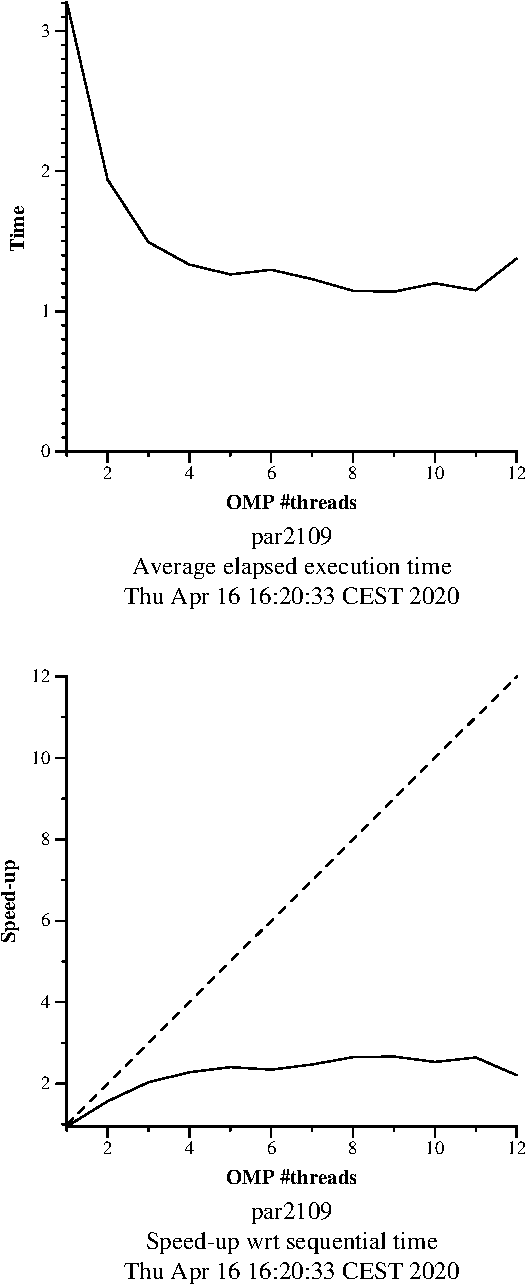
\includegraphics[width=0.7\linewidth]{plots/v1-crop.pdf}
        \caption{Strong scalability analysis v1}
        \label{fig:ssa_v1} 
    \end{minipage}
    \begin{minipage}{0.5\textwidth}
        \centering
        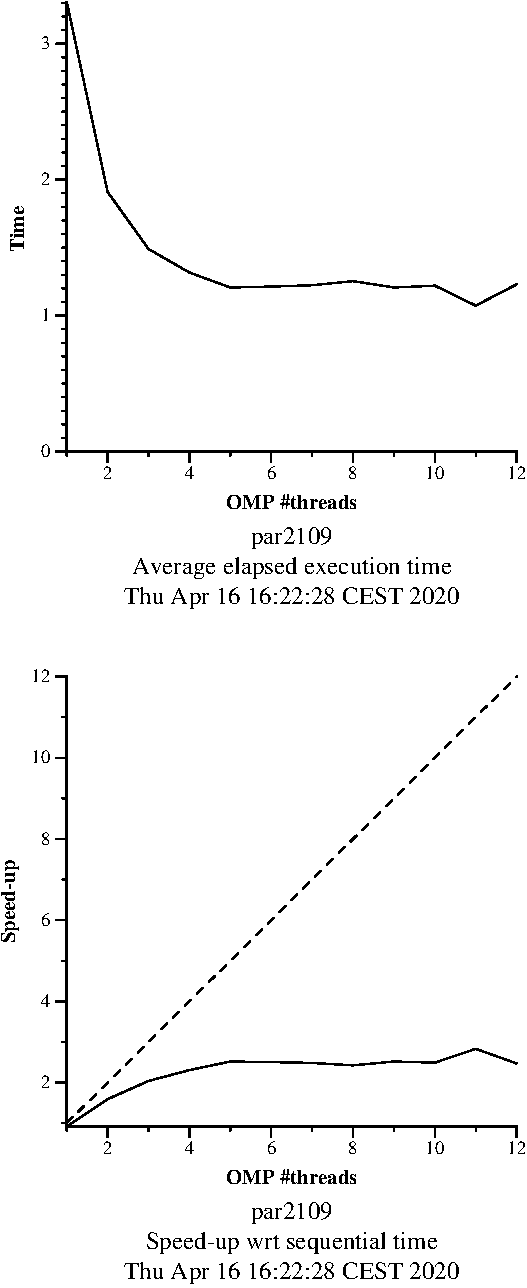
\includegraphics[width=0.7\linewidth]{plots/v2-crop.pdf}
        \caption{Strong scalability analysis v2}
        \label{fig:ssa_v2} 
    \end{minipage}
\end{figure}

\begin{figure}[H]
    \begin{minipage}{0.5\textwidth}
        \centering
        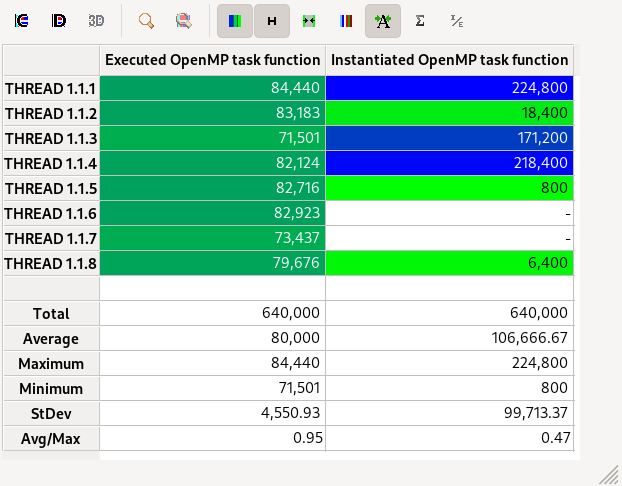
\includegraphics[width=0.7\linewidth]{captures/v1-profile.png}
        \caption{Paraver \texttt{tasks\_profile} v1}
        \label{fig:ssa_v1} 
    \end{minipage}
    \begin{minipage}{0.5\textwidth}
        \centering
        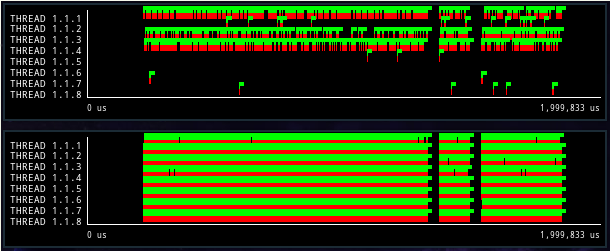
\includegraphics[width=\linewidth]{captures/v1-plot.png}
        \caption{Paraver tasks v1}
        \label{fig:ssa_v2} 
    \end{minipage}
\end{figure}

\begin{figure}[H]
    \begin{minipage}{0.5\textwidth}
        \centering
        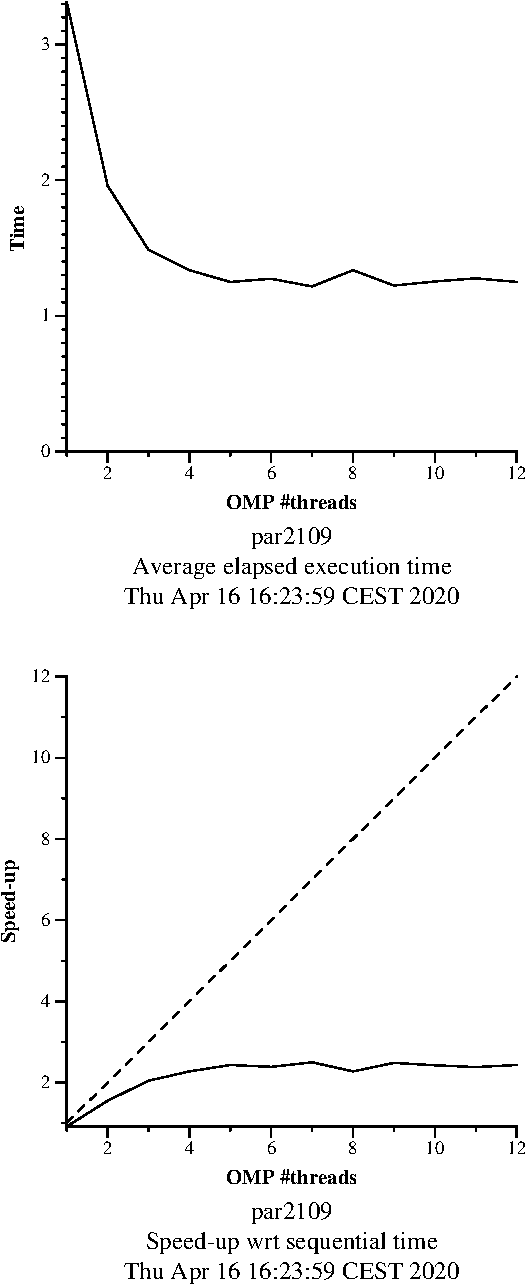
\includegraphics[width=0.7\linewidth]{plots/v3-crop.pdf}
        \caption{Strong scalability analysis v3}
        \label{fig:ssa_v3} 
    \end{minipage}
    \begin{minipage}{0.5\textwidth}
        \centering
        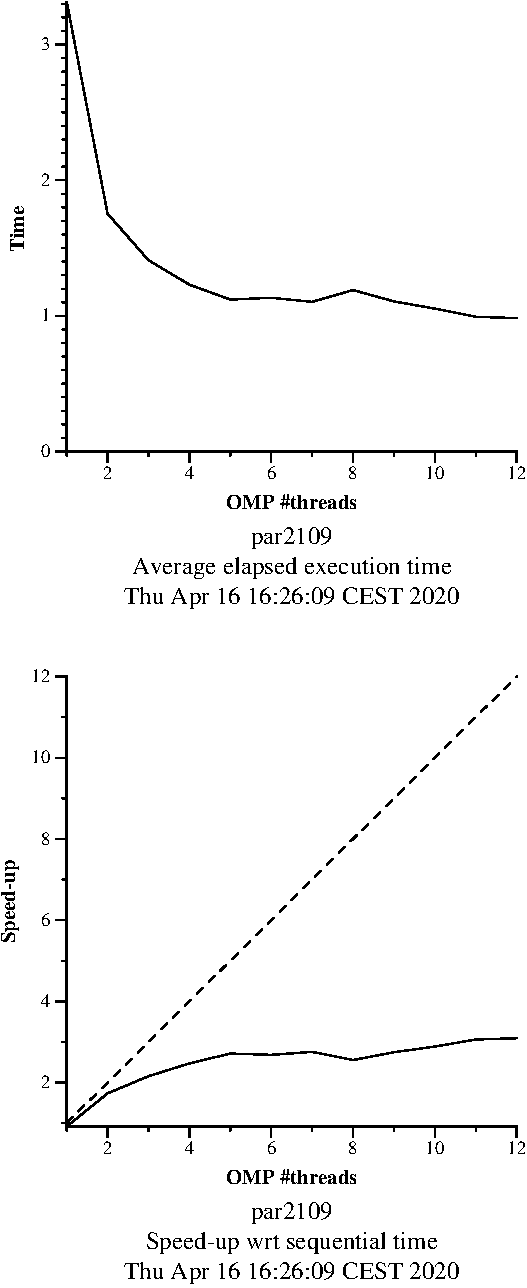
\includegraphics[width=0.7\linewidth]{plots/v4-crop.pdf}
        \caption{Strong scalability analysis v4}
        \label{fig:ssa_v4} 
    \end{minipage}
\end{figure}


\begin{figure}[H]
    \begin{minipage}{0.5\textwidth}
        \centering
        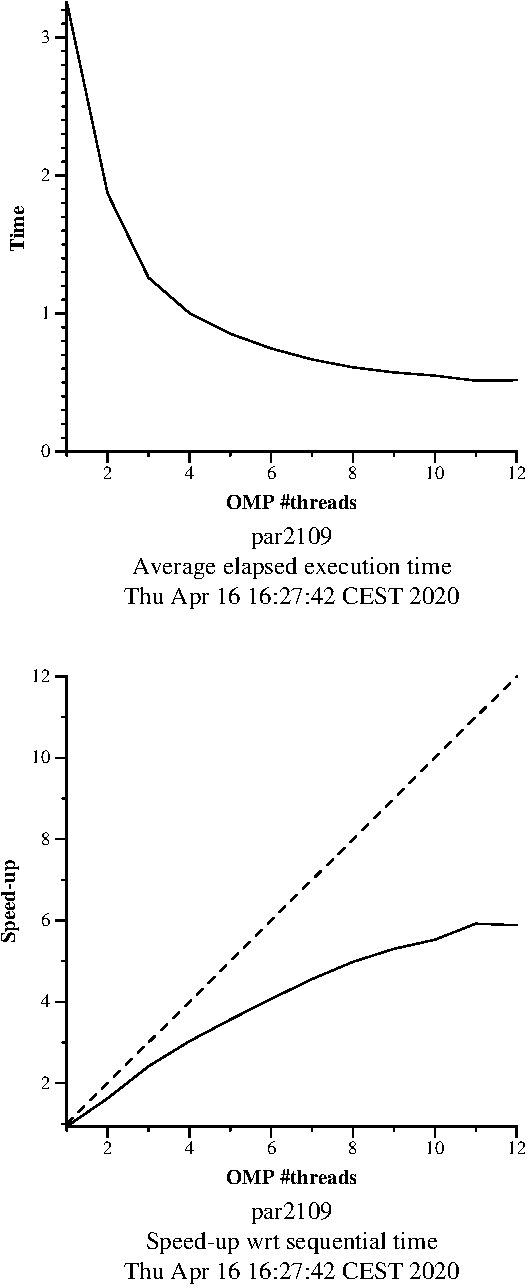
\includegraphics[width=0.7\linewidth]{plots/v5-crop.pdf}
        \caption{Strong scalability analysis v5}
        \label{fig:ssa_v5} 
    \end{minipage}
    \begin{minipage}{0.5\textwidth}
        \centering
        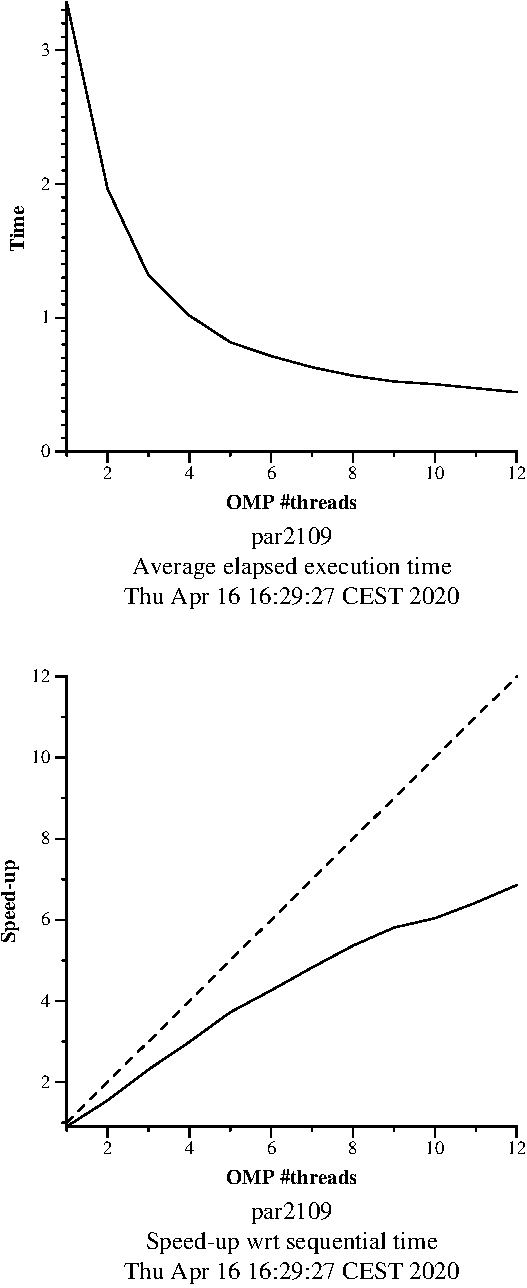
\includegraphics[width=0.7\linewidth]{plots/v6-crop.pdf}
        \caption{Strong scalability analysis v6}
        \label{fig:ssa_v6} 
    \end{minipage}
\end{figure}

\begin{figure}[H]
    \begin{minipage}{0.5\textwidth}
        \centering
        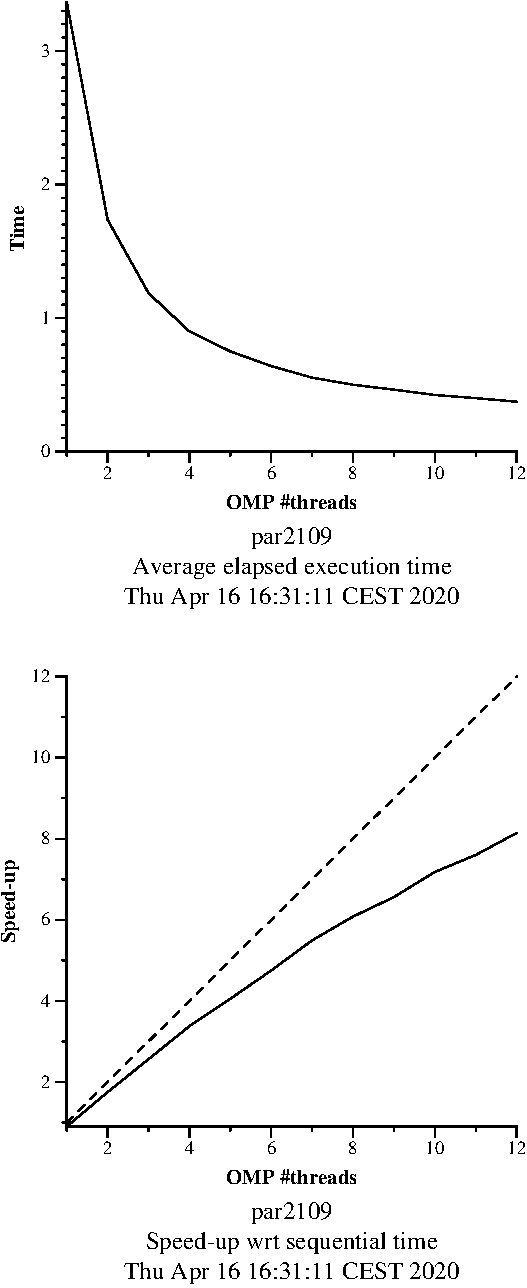
\includegraphics[width=0.7\linewidth]{plots/v7-crop.pdf}
        \caption{Strong scalability analysis v7}
        \label{fig:ssa_v7} 
    \end{minipage}
    \begin{minipage}{0.5\textwidth}
        \centering
        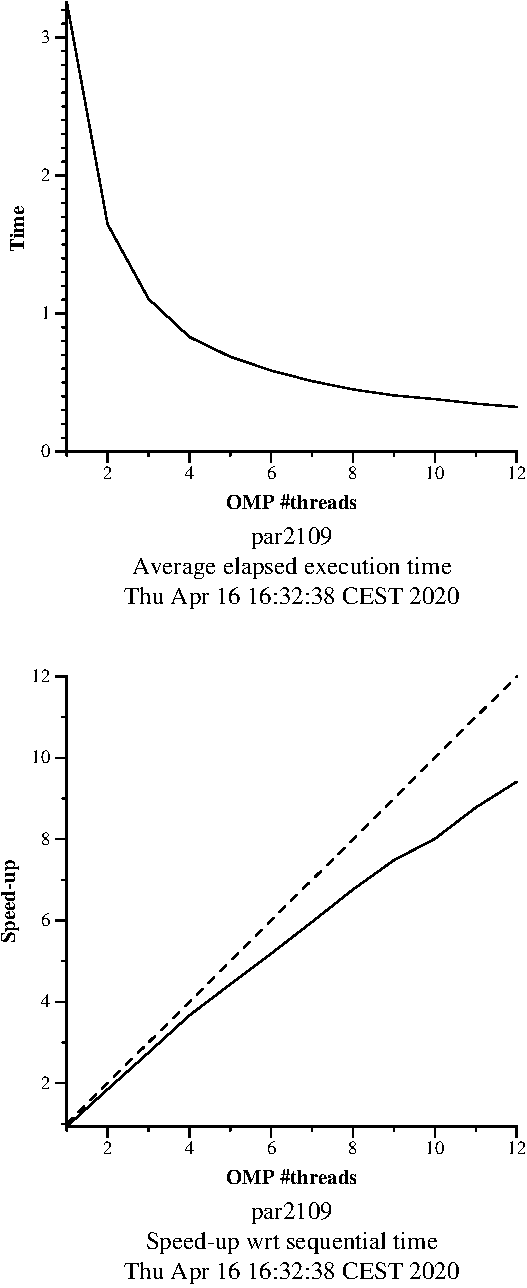
\includegraphics[width=0.7\linewidth]{plots/v8-crop.pdf}
        \caption{Strong scalability analysis v8}
        \label{fig:ssa_v8} 
    \end{minipage}
\end{figure}


\begin{table}[H]
    \caption{Execution times with different grainsizes}%
    \label{tab:grainsize}
    \begin{center}
    \begin{tabular}{lr}
\toprule
{} &      time \\
grainsize &           \\
\midrule
1         &  0.317474 \\
2         &  0.361412 \\
5         &  0.372336 \\
10        &  0.256939 \\
25        &  0.208336 \\
50        &  0.196701 \\
100       &  0.183566 \\
200       &  0.181784 \\
400       &  0.185489 \\
800       &  0.185322 \\
\bottomrule
\end{tabular}

    \end{center}
\end{table}

\begin{figure}[H]
    \centering
    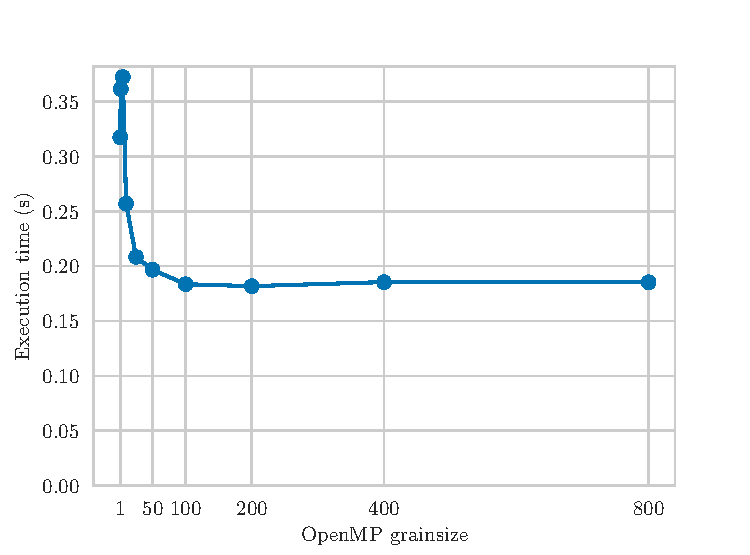
\includegraphics{plots/grainsize.pdf}
    \caption{Plot of execution time for different grainsizes}
    \label{fig:grain} 
\end{figure}

\begin{figure}[H]
    \centering
    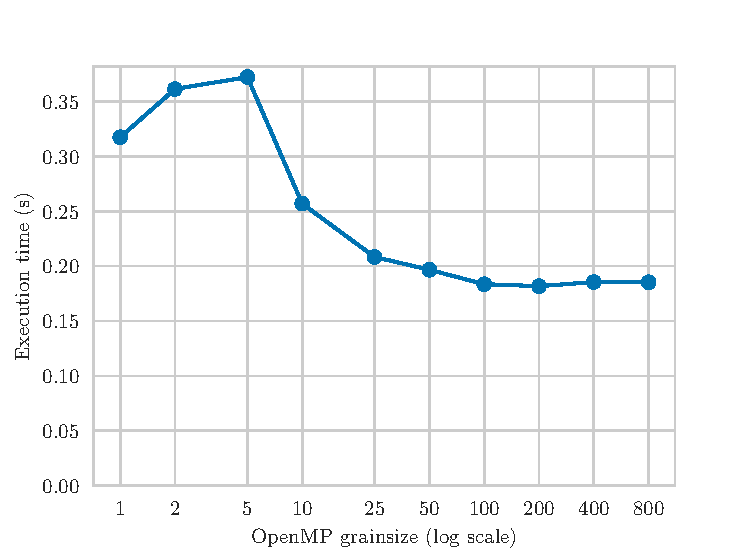
\includegraphics{plots/grainsize_log.pdf}
    \caption{Plot of execution time for different grainsizes (log scale)}
    \label{fig:grain_log} 
\end{figure}

\begin{figure}[H]
    \centering
    \caption{Mandel tar code}
    \inputminted[firstline=91,lastline=127]{c}{sources/mandel-tar.c}
    \vspace{-2em}
    \inputminted[firstline=200,lastline=210]{c}{sources/mandel-tar.c}
    \label{fig:grain_log} 
\end{figure}

\section{Conclusions}%
\label{sec:Conclusions}

% TODO: I aqui pues relleno bonito del final


\end{document}
